%%%%%%%%%%%%%%%%%%%%%%%%%%%
%%%%%%%%%%%%%%%%%%%%%%%%%%%
% title page
%%%%%%%%%%%%%%%%%%%%%%%%%%%
%%%%%%%%%%%%%%%%%%%%%%%%%%%

\begin{center}\bfseries\Huge WESTMINSTER ABBEY

\vspace{1in}


\includegraphics[width=2in]{arms.png}


THE STATE FUNERAL\\
of\\
HER MAJESTY\\
QUEEN ELIZABETH II\\

\vspace{1in}


\normalfont\tnr\LARGE Monday, 19th September, 2022\\
at 11.00 a.m.
\end{center}
\clearpage
 %%%%%%%%%%%%%%%%%%%%%%%%%%%
%%%%%%%%%%%%%%%%%%%%%%%%%%%
% disclaimer page
%%%%%%%%%%%%%%%%%%%%%%%%%%%
%%%%%%%%%%%%%%%%%%%%%%%%%%%\itshape
\color{qred}\itshape Members of the Congregation are kindly requested to refrain from using private cameras, video, or
sound recording equipment. Please ensure that mobile phones and other electronic devices are
switched off.

\vspace*{.5in}

The church is served by a hearing loop. Users should turn their hearing aid to the setting marked \normalfont T\itshape .


\vspace*{1in}

The service is conducted by The Very Reverend Dr David Hoyle \scalebox{0.72}{MBE}, Dean of Westminster.

\vspace*{.5in}


The service is sung by the Choir of Westminster Abbey and the Choir of the Chapel Royal,
St James’s Palace, (Joseph McHardy, Director of Music) under the direction of James O’Donnell,
Organist and Master of the Choristers, Westminster Abbey.

\vspace*{.5in}


The State Trumpeters of the Household Cavalry are led by Trumpet Major Julian Sandford.

The Fanfare Team of the Household Division Bands is conducted by Lieutenant Colonel David
Barringer \scalebox{0.72}{MBE}, Commanding Officer, Household Division Bands.

\vspace*{.5in}

The organ is played by Peter Holder, Sub-Organist, Westminster Abbey.


Before the service, the tenor bell is tolled every minute for 96 minutes, reflecting the years of
Queen Elizabeth II’s life.

\vspace*{.15in}

Members of Foreign Royal Families, Heads of State, and Overseas Government Representatives are
received at the Great West Door by the Dean and Chapter of Westminster and are conducted to their seats in the Lantern. All remain seated.

\vspace*{.15in}

Music before the service:\\%
Matthew Jorysz, Assistant Organist, Westminster Abbey, plays


  \begin{minipage}[t]{0.5\textwidth}
    \begin{flushleft}
\textcolor{black}{\normalfont%
Fantasia of four parts}
\end{flushleft}
\end{minipage}%
%
\begin{minipage}[t]{0.5\textwidth}
    \begin{flushright}
Orlando Gibbons (1583–1625)\\Organist of Westminster Abbey 1623–25
    \end{flushright}
\end{minipage}




\musictab{Romanza (Symphony no 5 in D)}{Ralph Vaughan Williams (1872–1958)}{
arranged by Robert Quinney (b 1976)}

\musictab{Reliqui domum meum}{Peter Maxwell Davies (1934–2016)}{}

\musictab{Meditation on ‘Brother James’s Air’}{Harold Darke (1888–1976)}{}

\musictab{Prelude on ‘Ecce jam noctis’ Op 157 no 3}{Healey Willan (1880–1968}{}

\musictab{Psalm Prelude Set 1 no 2}{Herbert Howells (1892–1983)}{}

\musictab{In the Country Op 194 no 2}{Charles Villiers Stanford (1852–1924)}{}

\musictab{Fantasy on ‘O Paradise’}{Malcolm Williamson (1931–2003)}{}

\musictab{Elegy Op 58}{Edward Elgar (1857–1934)}{
arranged by Matthew Jorysz (b 1992)}

The Sub-Organist plays\\\musictab{Andante espressivo (Sonata in G Op 28)}{Edward Elgar}{}

\musictab{Sospiri Op 70}{Edward Elgar}{arranged by Peter Holder (b 1990)}

The Procession of Religious Representatives moves to places in the Nave and the Sacrarium. All
remain seated.

\proc{Verger}{}\vspace{-.25in}\proc{Mrs Marie van der Zyl}{President, Board of Deputies of British Jews}

\proc{Dr Shirin Fozdar-Faroudi}{Representative of the Bahá’í Community}

\proc{Mr Nemu Chandaria \textcsc{OBE}}{
Representative of the Jain Community}
\proc{Mr Malcolm Deboo}{Representative of the Zoroastrian Community}

\proc{The Venerable Bogoda Seelawimala}{Representative of the Buddhist Community}

\proc{The Lord Singh of Wimbledon \textcsc{CBE}}{Representative of the Sikh Community}

\proc{Mr Rajnish Kashyap}{General Secretary, Hindu Council UK}

\proc{Mrs Aliya Azam \textcsc{MBE}}{Interfaith Co-ordinator, Al-Khoei Foundation}

\proc{Shaykh Dr Asim Yusuf}{Muslim Scholar}

\proc{Chief Rabbi Ephraim Mirvis}{Chief Rabbi of Great Britain and the United Hebrew Congregations of the Commonwealth}

\vspace*{0.5in}

\begin{center}
\normalfont\color{black}	Verger
\end{center}
\begin{center}\normalfont\scshape Representing the Churches of
Wales\end{center}

\proc{The Reverend Simon Walkling}{President, Free Church Council of Wales}

\begin{minipage}[t]{.5\textwidth}\proc{The Most Reverend Andrew John}{Archbishop of Wales}	
\end{minipage}%
%
\begin{minipage}[t]{.5\textwidth}
\proc{The Most Reverend Mark O’Toole}{Archbishop of Cardiff}
\end{minipage}

\medskip

\begin{center}\normalfont
\textsc{Representing the Churches of Scotland}\end{center}


\proc{The Right Reverend Dr Iain Greenshields}{Moderator of the General Assembly of the Church of Scotland}

\begin{minipage}[t]{.5\textwidth}\proc{The Most Reverend Leo Cushley}{Archbishop of St Andrews and Edinburgh}
\end{minipage}
%
\begin{minipage}[t]{.5\textwidth}
\proc{The Most Reverend Mark Strange}{Primus, Scottish Episcopal Church}
\end{minipage}


\begin{center}
\normalfont\textsc{Representing the Churches of Northern Ireland}\end{center}

\begin{minipage}[t]{.5\textwidth}
\proc{The Reverend David Nixon}{President,\\Methodist Church in Ireland}
\end{minipage}
\begin{minipage}[t]{.5\textwidth}
\proc{The Reverend Ian Brown}{Lead Minister, Martyrs Memorial\\Free Presbyterian Church}
\end{minipage}

\proc{The Right Reverend Dr John Kirkpatrick}{Moderator, The Presbyterian Church in Ireland}




\begin{minipage}[t]{.5\textwidth}
\proc{The Most Reverend Dr Eamon Martin}
{Archbishop of Armagh\\
and Primate of All Ireland}
\end{minipage}
\begin{minipage}[t]{.5\textwidth}
\proc{The Most Reverend John McDowell}{Archbishop of Armagh and Primate\\
of All Ireland and Metropolitan}
\end{minipage}

\begin{center}\normalfont
\textsc{Representing the Churches in England}\end{center}


\begin{minipage}[t]{.5\textwidth}\proc{
Pastor Agu Irukwu}
{Senior Pastor, Jesus House UK}\end{minipage}
\begin{minipage}[t]{.5\textwidth}\proc{
Pastor Glyn Barrett}{
National Leader, Assemblies of God}\end{minipage}

\begin{minipage}[t]{.5\textwidth}\proc{
The Reverend Canon Helen Cameron}{
Moderator, Free Churches Group}\end{minipage}
\begin{minipage}[t]{.5\textwidth}\proc{
Ms Shermara Fletcher}{
Principal Officer for Pentecostal\\
and Charismatic Relations,\\
Churches Together in England}\end{minipage}


\begin{minipage}[t]{.5\textwidth}\proc{
The Reverend Canon
Graham Thompson}{
President, Methodist Conference}\end{minipage}
\begin{minipage}[t]{.5\textwidth}\proc{
His Eminence
Archbishop Angaelos}{
The Coptic Church in Great Britain}\end{minipage}

\begin{minipage}[t]{.5\textwidth}\proc{
His Eminence Cardinal Vincent Nichols}{
Archbishop of Westminster}\end{minipage}
\begin{minipage}[t]{.5\textwidth}\proc{
His Eminence Archbishop Nikitas}
{Archbishop of Thyateira and Great Britain}
\end{minipage}

\proc{Serjeant of the Vestry}{}
\vspace{-.15in}
\proc{
The Very Reverend Professor David Fergusson \textcsc{OBE}}{
Dean of the Thistle and of the Chapel Royal in Scotland}

\proc{The Reverend Canon Paul Wright}{Sub-Dean of His Majesty’s Chapels Royal}

\proc{The Right Reverend and Right Honourable Dame Sarah Mullally \textcsc{DBE}}{
Bishop of London and Dean of His Majesty’s Chapels Royal}

\proc{The Right Reverend David Conner \textcsc{KCVO}}{
Dean of Windsor}

\proc{The Right Reverend James Newcome}{
Clerk of the Closet}

\proc{The Right Reverend Dr John Inge}{
Lord High Almoner}

Members of the Royal Family are received at the Great West Door by the Dean and Chapter of
Westminster and are conducted to their seats in the Lantern. All remain seated.


The Choir of Westminster Abbey and the Choir of the Chapel Royal, St James’s Palace, proceed to
places in the Nave and in Quire. All remain seated.\begin{center}
\normalfont\color{black}\LARGE\addfontfeature{LetterSpace=25} ORDER OF SERVICE
\end{center}

All stand as the Procession of the Coffin enters the Abbey.



The Choir of Westminster Abbey sings
\begin{center}\normalfont\bfseries
THE SENTENCES
\end{center}
during which the Procession of the Coffin moves through the Abbey

\sntnc{I}{ am}{ the resurrection and the life, saith the Lord: he that believeth in me, though he
were dead, yet shall he live: and whosoever liveth and believeth in me shall never
die.}{John 11: 25–26}

\sntnc{I}{ know}{ that my Redeemer liveth, and that he shall stand at the latter day upon the
earth: and though after my skin worms destroy this body, yet in my flesh shall I see
God; whom I shall see for myself, and mine eyes shall behold, and not another.}{Job 19: 25–27}

\color{black}\normalfont \lettrine[lines=2,loversize=.2]{W}{e} brought nothing into this world, and it is certain we can carry nothing out.\\The Lord gave, and the Lord hath taken away; blessed be the name of the Lord.\color{qred}\itshape\\
William Croft (1678–1727)\hfill 1 Timothy 6: 7; Job 1: 21\\
Organist of Westminster Abbey 1708–27



The Choir of Westminster Abbey and the Choir of the Chapel Royal, St James’s Palace, sing

\color{black}\normalfont \lettrine[lines=2,loversize=.2]{T}{hou} knowest, Lord, the secrets of our hearts; shut not thy merciful ears unto our
prayer; but spare us, Lord most holy, O God most mighty, O holy and most
merciful Saviour, thou most worthy Judge eternal, suffer us not, at our last hour, for
any pains of death, to fall from thee. \textbf{Amen}.\\\itshape\color{qred}
Henry Purcell (1659–95)\hfill The Book of Common Prayer 1549\\
Organist of Westminster Abbey 1679–95


\color{black}\normalfont \lettrine[lines=2,loversize=.2]{I}{ 
heard} a voice from heaven, saying unto me, Write, From henceforth blessed are
the dead which die in the Lord: even so saith the Spirit; for they rest from their
labours. \textbf{Amen}.\\\itshape\color{qred}
William Croft\hfill Revelation 14: 13

\begin{center}\normalfont\color{black}
	
Beadle

The Choir of Westminster Abbey

\proc{
Mr James O’Donnell}{
Organist and Master of the Choristers}



{\itshape\color{qred}Pursuivants and Heralds of Arms of Scotland:}

\begin{minipage}[t]{0.35\textwidth}\begin{center}
March

Linlithgow

Ormond

Rothesay\end{center}\end{minipage}\begin{minipage}[t]{0.35\textwidth}\begin{center}
Falkland 

Unicorn 

Carrick 

Marchmont	
\end{center}\end{minipage}

{\itshape\color{qred}Pursuivants and Heralds of Arms of England:}
\begin{minipage}[t]{0.35\textwidth}\begin{center}
Portcullis 

Rouge Dragon 

Norfolk

Windsor\end{center}\end{minipage}%
\begin{minipage}[t]{0.35\textwidth}\begin{center}

Bluemantle 

Wales


 Maltravers	
 
 York\end{center}
\end{minipage}

Richmond



{\itshape\color{qred}Kings of Arms:}


\begin{minipage}[t]{0.25\textwidth}\begin{center}
Norroy and Ulster\\
King of Arms\end{center}\end{minipage}
\begin{minipage}[t]{0.25\textwidth}\begin{center}
Lord Lyon\\
King of Arms\end{center}\end{minipage}
\begin{minipage}[t]{0.25\textwidth}\begin{center}
Clarenceux\\
King of Arms
\end{center}\end{minipage}

\begin{minipage}[t]{0.25\textwidth}\begin{center}
Lady Usher\\
of the Black Rod
\end{center}\end{minipage}
\begin{minipage}[t]{0.25\textwidth}\begin{center}
\end{center}\end{minipage}
\begin{minipage}[t]{0.25\textwidth}\begin{center}
Garter Principal\\
King of Arms\end{center}\end{minipage}

{\color{qred}\itshape Household of Queen Elizabeth II:}

\hrld{Master of the Horse}{}\begin{minipage}[t]{0.15\textwidth}\begin{center}
\end{center}\end{minipage}
\hrld{Lord Steward}{}

\hrld{Director of the}{
Royal Collection}
\althrld{Comptroller,}{Lord Chamberlain’s Office}
\hrld{Master of the}{
Household}{}



\althrld{Keeper of the Privy Purse}{}\begin{minipage}[t]{0.1\textwidth}\begin{center}
\end{center}\end{minipage}
\althrld{Private Secretary
}{}

\hrld{The Queen’s Page}{}
\hrld{The Queen's Page,}{}
\hrld{Palace Steward}{}

\proc{Verger}{}
\proc{The King’s Almsmen}{}
\proc{Verger}{}
\splitproc{Primatial Cross of York}{}{Primatial Cross of Canterbury}{}
\splitproc{The Most Reverend and Right
Honourable Stephen Cottrell}{
Archbishop of York,
Primate of England and Metropolitan}{The Most Reverend and Right\\
Honourable Justin Welby}{
Archbishop of Canterbury,
Primate of All England and Metropolitan}
\proc{The Cross of Westminster and Lights}{}
\splitproc{The Reverend Robert Latham}{Minor Canon and Sacrist}{The Reverend Mark Birch}{Minor Canon and Precentor}
\proc{Mr Paul Baumann \textcsc{CBE}}
{Receiver General}
\proc{Sir Kenneth Olisa \textcsc{OBE}}{High Bailiff of Westminster}
\end{center}


\proc{Verger}{}
\splitproc{The Venerable Tricia Hillas}
{Canon Steward and
Archdeacon of Westminster}
{The Reverend Dr James Hawkey}
{Canon Theologian
and Almoner}

\splitproc{The Right Reverend Anthony Ball}{Canon of Westminster and
Rector of St Margaret’s Church}{The Reverend David Stanton}{Sub-Dean and
Canon Treasurer}
\proc{Dean’s Verger}{}
\proc{The Very Reverend Dr David Hoyle \textcsc{MBE}}
{Dean of Westminster}

\splitproc{Pall Bearers}{}{Pall Bearers}{}

\splitproc{Lord Chamberlain}{}{Earl Marshal}{}

\proc{{\addfontfeature{LetterSpace=10}HER MAJESTY’S COFFIN}}{surmounted by\\\normalfont
The Imperial State Crown,\\
The Orb and The Sceptre\\\itshape
and borne by the\\\normalfont Bearer Party}

\splitproc{
The Queen Consort}{}{{\addfontfeature{LetterSpace=10}THE KING}}{}\\
\splitproc{Vice Admiral Sir Tim Laurence}{}{The Princess Royal}{}\\
\proc{The Duke of York}{}
\splitproc{The Countess of Wessex and Forfar}{}{The Earl of Wessex and Forfar}{}\\
\splitproc{The Princess of Wales}{}{The Prince of Wales}{}\\
\splitproc{Princess Charlotte of Wales}{}
{Prince George of Wales}{}\\
\splitproc{The Duchess of Sussex}{}
{The Duke of Sussex}{}
\\
\splitproc{The Earl of Snowdon}{}{Mr Peter Phillips}{}\\
\proc{The Duke of Gloucester}{}\\
\splitproc{Prince Michael of Kent}{}{The Duke of Kent}{}

Household of The former Prince of Wales and Duchess of Cornwall:

\splitproc{Private Secretary}{}{Principal Private Secretary}{}\\\splitproc{Equerry}{}{Master of the Household}{}

Household of The Prince and Princess of Wales:

\proc{Equerry}
All remain standing. The Very Reverend Dr David Hoyle \scalebox{0.72}{MBE}, Dean of Westminster, gives

\begin{center}
\normalfont\bfseries\addfontfeature{LetterSpace=10} THE BIDDING
\end{center}


\color{black}\normalfont
\mylett{I}{N}  grief and also in profound thanksgiving we come to this House of God, to a place
of prayer, to a church where remembrance and hope are sacred duties. Here, where
Queen Elizabeth was married and crowned, we gather from across the nation, from the
Commonwealth, and from the nations of the world, to mourn our loss, to remember
her long life of selfless service, and in sure confidence to commit her to the mercy of
God our maker and redeemer.

With gratitude we remember her unswerving commitment to a high calling over so
many years as Queen and Head of the Commonwealth. With admiration we recall her
life-long sense of duty and dedication to her people. With thanksgiving we praise God
for her constant example of Christian faith and devotion. With affection we recall her
love for her family and her commitment to the causes she held dear.


Now, in silence, let us in our hearts and minds recall our many reasons for thanksgiving,
pray for all members of her family, and commend Queen Elizabeth to the care and
keeping of almighty God.\\\itshape\color{qred}
A brief silence is kept.

\color{black}\normalfont\mylett{O}{MERCIFUL} God, the Father of our Lord Jesus Christ, who is the resurrection
and the life; in whom whosoever believeth shall live, though he die; and
whosoever liveth, and believeth in him, shall not die eternally; who hast taught us, by
his holy Apostle Saint Paul, not to be sorry, as men without hope, for them that sleep
in him: We meekly beseech thee, O Father, to raise us from the death of sin unto the
life of righteousness; that, when we shall depart this life, we may rest in him, as our
hope is this our sister doth; and that, at the general Resurrection in the last day, we may
be found acceptable in thy sight; and receive that blessing, which thy well-beloved Son
shall then pronounce to all that love and fear thee, saying, Come, ye blessed children of
my Father, receive the kingdom prepared for you from the beginning of the world.
Grant this, we beseech thee, O merciful Father, through Jesus Christ, our mediator and
redeemer. \textbf{Amen}.

All sing

\begin{center}
	\bfseries\color{qred}THE HYMN

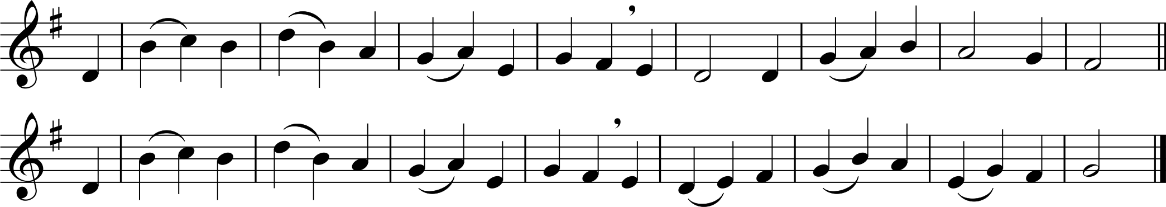
\includegraphics[width=.8\textwidth]{hymn1.png}

\color{black}\normalfont
\mylett{T}{HE} day thou gavest, Lord, is ended,\\
the darkness falls at thy behest;\\
to thee our morning hymns ascended,\\
thy praise shall sanctify our rest.

We thank thee that thy Church unsleeping,\\
while earth rolls onward into light,\\
through all the world her watch is keeping,\\
and rests not now by day or night.

As o’er each continent and island\\
the dawn leads on another day,\\
the voice of prayer is never silent,\\
nor dies the strain of praise away.

The sun that bids us rest is waking\\
our brethren ’neath the western sky,\\
and hour by hour fresh lips are making\\
thy wondrous doings heard on high.

So be it, Lord; thy throne shall never,\\
like earth’s proud empires, pass away;\\
thy kingdom stands, and grows for ever,\\ 
till all thy creatures own thy sway.
\end{center}

{\color{qred}\itshape St Clement\hfill John Ellerton (1826–93)\\
Clement Scholefield (1839–1904)\\
arranged by James O’Donnell (b 1961)
}
{\color{qred}\itshape All sit. The Right Honourable the Baroness Scotland of Asthal KC, Secretary-General of the
Commonwealth, reads}

\begin{center}\bfseries\color{qred}
	THE FIRST LESSON

\end{center}

\mylett{N}{OW} is Christ risen from the dead, and become the firstfruits of them that slept.
For since by man came death, by man came also the resurrection of the dead. For
as in Adam all die, even so in Christ shall all be made alive. But every man in his own
order: Christ the firstfruits; afterward they that are Christ’s at his coming. Then cometh
the end, when he shall have delivered up the kingdom to God, even the Father; when
he shall have put down all rule and all authority and power. For he must reign, till he
hath put all enemies under his feet. The last enemy that shall be destroyed is death. For
this corruptible must put on incorruption, and this mortal must put on immortality. So
when this corruptible shall have put on incorruption, and this mortal shall have put on
immortality, then shall be brought to pass the saying that is written, Death is swallowed
up in victory. O death, where is thy sting? O grave, where is thy victory? The sting of
death is sin; and the strength of sin is the law. But thanks be to God, which giveth us
the victory through our Lord Jesus Christ. Therefore, my beloved brethren, be ye
steadfast, unmoveable, always abounding in the work of the Lord, forasmuch as ye
know that your labour is not in vain in the Lord.

\hfill {\itshape\color{qred}1 Corinthians 15: 20–26, 53–end}

Thanks be to God.


\qred{All remain seated. The choir sings}


\begin{center}
	\bfseries\color{qred} THE PSALM
\end{center}

\mylett{L}{IKE} as the hart desireth the water-brooks : so longeth my soul after thee, O God.
My soul is athirst for God, yea, even for the living God : when shall I come to
appear before the presence of God?
My tears have been my meat day and night : while they daily say unto me, Where is
now thy God?
Now when I think thereupon, I pour out my heart by myself : for I went with the
multitude, and brought them forth into the house of God;
In the voice of praise and thanksgiving : among such as keep holy-day.
Why art thou so full of heaviness, O my soul : and why art thou so disquieted within
me?
Put thy trust in God : for I will yet give him thanks for the help of his countenance.
Judith Weir CBE (b 1954)
composed for this Service

Psalm 42: 1–7

{\color{qred}\itshape The Right Honourable Elizabeth Truss MP, Prime Minister of the United Kingdom of Great Britain
and Northern Ireland, reads
}

\serv{THE SECOND LESSON}

\mylett{L}{ET} not your heart be troubled: ye believe in God, believe also in me. In my Father’s
house are many mansions: if it were not so, I would have told you. I go to prepare
a place for you. And if I go and prepare a place for you, I will come again, and receive
you unto myself; that where I am, there ye may be also. And whither I go ye know, and
the way ye know. Thomas saith unto him, Lord, we know not whither thou goest; and
how can we know the way? Jesus saith unto him, I am the way, the truth, and the life:
no man cometh unto the Father, but by me. If ye had known me, ye should have known
my Father also: and from henceforth ye know him, and have seen him. Philip saith unto
him, Lord, shew us the Father, and it sufficeth us. Jesus saith unto him, Have I been so
long time with you, and yet hast thou not known me, Philip? He that hath seen me hath
seen the Father.
John 14: 1–9a

Thanks be to God.


\qred{All stand to sing}

\serv{THE HYMN}

\begin{center}
	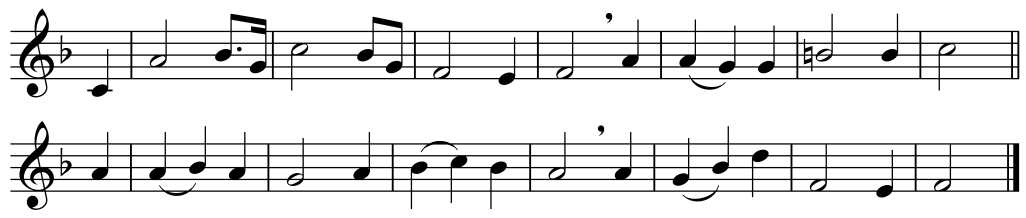
\includegraphics[width=.8\textwidth]{hymn2.png}

\end{center}

\begin{center}

\mylett{T}{HE} Lord’s my shepherd, I’ll not want;\\
he makes me down to lie\\
in pastures green; he leadeth me\\
the quiet waters by.

My soul he doth restore again,\\
and me to walk doth make\\
within the paths of righteousness,\\
e’en for his own name’s sake.
\end{center}


\begin{minipage}[t]{0.3\textwidth}
\begin{flushleft}
\textcolor{qred}{\textit{The choir sings}}
\end{flushleft}
\end{minipage}\begin{minipage}[t]{0.7\textwidth}
\begin{flushleft}
Yea, though I walk through death’s dark vale\end{flushleft}
\end{minipage}\vspace{-.7em}\begin{center}
yet will I fear none ill;\\ for thou art with me, and thy rod\\
and staff me comfort still.\end{center}

\begin{tabular}{@{}l@{}p{3.75in}r@{}}
\qred{All sing}&\centering My table thou hast furnishèd&\end{tabular}\\\vspace{-2em}\begin{center}
in presence of my foes;\\
my head thou dost with oil anoint,\\ 
and my cup overflows.

Goodness and mercy all my life\\
shall surely follow me;\\
and in God’s house for evermore\\
my dwelling place shall be.\\
\end{center}


\qred{
Crimond\hfill Psalm 23\\
attributed to Jessie Seymour Irvine (1836–87)\hfill in {\normalfont Scottish Psalter} 1650\\
harmony by David Grant (1833–93)\\
descant by William Baird Ross (1871–1950)\\
}

\serv{THE SERMON}

\proc{The Most Reverend and Right Honourable Justin Welby}{\color{qred}Archbishop of Canterbury, Primate of All England and Metropolitan}

\vspace{0.25in}

{\color{qred}\itshape All remain seated. The choir sings}

\serv{THE ANTHEM}

\begin{center}
	
\raisebox{1ex}{\begin{minipage}{0.5\textwidth}%
	\mylett{M}{Y} soul, there is a country\\
Far beyond the stars,\\
Where stands a wingèd sentry\\
All skilful in the wars:

There above noise, and danger,\\
Sweet Peace sits crowned with smiles,\\
And One born in a manger\\
Commands the beauteous files.

\end{minipage}}\raisebox{.25ex}{\begin{minipage}{0.5\textwidth}%
He is thy gracious friend,\\
And (O my soul, awake!)\\
Did in pure love descend,\\To die here for thy sake.

If thou canst get but thither,\\
There grows the flower of Peace,\\
The Rose that cannot wither,\\
Thy fortress, and thy ease.
\end{minipage}}
\end{center}

\begin{center}
	Leave then thy foolish ranges,\\
For none can thee secure,\\
But One who never changes,\\
Thy God, thy Life, thy Cure.\\
\end{center}

\qred{from Songs of Farewell\hfill Henry Vaughan (1621–95)\\
Hubert Parry (1848–1918)}


\qred{The Reverend Mark Birch, Minor Canon and Precentor, leads}


\serv{THE PRAYERS}

In confidence and trust, let us pray to the Father.


\qred{All kneel or remain seated.\\
The Reverend Dr Iain Greenshields, Moderator of the General Assembly of the Church of Scotland,
says}


Let us give thanks to God for Queen Elizabeth’s long life and reign, recalling with
gratitude her gifts of wisdom, diligence, and service.

\mylett{O}{ GOD}, from whom cometh everything that is upright and true: accept our thanks
for the gifts of heart and mind that thou didst bestow upon thy daughter
Elizabeth, and which she showed forth among us in her words and deeds; and grant that
we may have grace to live our lives in accordance with thy will, to seek the good of
others, and to remain faithful servants unto our lives’ end; through Jesus Christ our
Lord. \textbf{Amen}.


\qred{Ms Shermara Fletcher, Principal Officer for Pentecostal and Charismatic Relations, Churches
Together in England, says}

Confident in God’s love and compassion, let us pray for all those whose hearts are heavy
with grief and sorrow.

\mylett{A}{LMIGHTY} God, Father of all mercies and giver of all comfort: deal graciously,
we pray thee, with those who mourn, that casting every care on thee, they may
know the consolation of thy love; through Jesus Christ our Lord. \textbf{Amen}.


\qred{The Right Reverend and Right Honourable Dame Sarah Mullally \scalebox{0.72}{DBE}, Bishop of London and
Dean of His Majesty’s Chapels Royal, says}

Let us pray for His Majesty The King and all the Royal Family; that they may know the
sustaining power of God’s love and the prayerful fellowship of God’s people.

\mylett{A}{LMIGHTY} God, the fountain of all goodness, we humbly beseech thee to bless
our most gracious Sovereign Lord King Charles, Camilla The Queen Consort,
William Prince of Wales, and all the Royal Family: endue them with thy Holy Spirit,
enrich them with thy heavenly grace; prosper them with all happiness; and bring them
to thine everlasting kingdom; through Jesus Christ our Lord. \textbf{Amen}.


\qred{The Reverend Canon Helen Cameron, Moderator of the Free Churches Group, says}

In recognition of Queen Elizabeth’s service to this United Kingdom, let us rejoice in
her unstinting devotion to duty, her compassion for her subjects, and her counsel to her
ministers; and we pray for the continued health and prosperity of this Nation.

\mylett{A}{LMIGHTY} God, whose will it is that all thy children should serve thee in serving
one another: look with love, we pray thee, on this Nation. Grant to its citizens
grace to work together with honest and faithful hearts, each caring for the good of all;
that, seeking first thy kingdom and its righteousness, they may possess all things needful
for their daily sustenance and the common good; through Jesus Christ our Lord.
Amen.

\qred{His Eminence Cardinal Vincent Nichols, Archbishop of Westminster, says}


Let us give thanks for Queen Elizabeth’s commitment to the Commonwealth
throughout her reign, for her service and dedication to its peoples, and for the rich
bonds of unity and mutual support she sustained.

\qred{O}{ ALMIGHTY} and everlasting God, hear our prayer for the Commonwealth, and
grant it the guidance of thy wisdom. Inspire those in authority, that they may
promote justice and the common good; give to all its citizens the spirit of mutual honour
and respect; and grant to us all grace to strive for the establishment of righteousness
and peace; for the honour of thy name. \textbf{Amen}.


\qred{The Most Reverend and Right Honourable Stephen Cottrell, Archbishop of York, Primate of
England and Metropolitan, says}

We give thanks to God for Queen Elizabeth’s loyalty to the faith she inherited through
her baptism and confirmation, and affirmed at her coronation; for her unswerving
devotion to the Gospel; and for her steadfast service as Supreme Governor of the
Church of England.

\mylett{L}{ORD}, we beseech thee to keep thy household the Church in continual godliness;
that through thy protection she may be free from all adversities, and devoutly
given to serve thee in all good works, to the glory of thy name; through Jesus Christ
our Lord. \textbf{Amen}.

\qred{The Precentor says}

Let us pray that we may be given grace to live as those who believe in the communion
of saints, the forgiveness of sins, and the resurrection to eternal life.

\mylett{B}{RING} us, O Lord God, at our last awakening into the house and gate of heaven, to
enter into that gate and dwell in that house, where there shall be no darkness nor
dazzling, but one equal light; no noise nor silence, but one equal music; no fears nor
hopes, but one equal possession; no ends nor beginnings, but one equal eternity; in the
habitation of thy glory and dominion, world without end. \textbf{Amen}.\\
\hfill\qred{John Donne (1572–1631)}

\qred{The choir sings}

\begin{center}
	
\mylett{O}{ TASTE} and see how gracious the Lord is:\\
blest is the man that trusteth in him.
\end{center}



\qred{Ralph Vaughan Williams\hfill Psalm 34: 8\\
composed for the Coronation of Queen Elizabeth II, 1953
}


\qred{The Precentor concludes}

In confidence and hope, let us pray to the Father in the words our Saviour taught us,

\mylett{O}{\bfseries UR}\bfseries\ Father, who art in heaven, hallowed be thy name; thy kingdom
come; thy will be done; on earth as it is in heaven. Give us this day
our daily bread. And forgive us our trespasses, as we forgive those who
trespass against us. And lead us not into temptation; but deliver us from
evil. For thine is the kingdom, the power, and the glory, for ever and ever.\\
Amen.\normalfont

\qred{All stand to sing}

\serv{THE HYMN}

\begin{center}

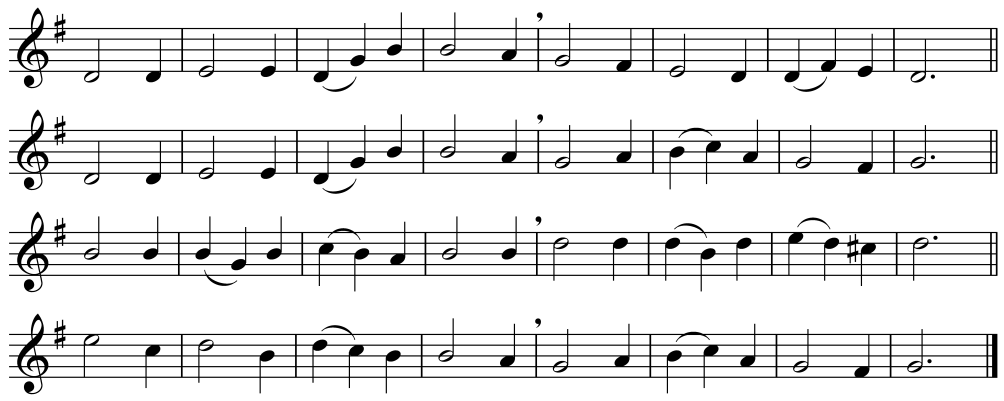
\includegraphics[width=.8\textwidth]{hymn3.png}

\mylett{L}{OVE} divine, all loves excelling,\\
\qquad joy of heaven, to earth come down,\\
fix in us thy humble dwelling,\\
all thy faithful mercies crown.\\
Jesu, thou art all compassion,\\
pure unbounded love thou art;\\
visit us with thy salvation,\\
enter every trembling heart.\\

Come, almighty to deliver,\\
let us all thy life receive;\\
suddenly return, and never,\\
never more thy temples leave.\\
Thee we would be always blessing,\\
serve thee as thy hosts above,\\
pray, and praise thee, without ceasing,\\
glory in thy perfect love.\\
Finish then thy new creation,\\
pure and spotless let us be;\\
let us see thy great salvation,\\
perfectly restored in thee,\\
changed from glory into glory\\
till in heaven we take our place,\\
till we cast our crowns before thee,\\
lost in wonder, love, and praise!
\end{center}
\qred{Blaenwern\hfill 
William Rowlands (1860–1937)\\Charles Wesley (1707–88)\\
arranged by James O’Donnell
}

\qred{All remain standing for}

\serv{THE COMMENDATION}

\qred{The Archbishop of Canterbury says}


Let us commend to the mercy of God, our maker and redeemer, the soul of Elizabeth, our late Queen.

\mylett{H}{EAVENLY} Father, King of kings, Lord and giver of life, who of thy grace in
creation didst form mankind in thine own image, and in thy great love offerest
us life eternal in Christ Jesus; claiming the promises of thy most blessed Son, we entrust
the soul of Elizabeth, our sister here departed, to thy merciful keeping, in sure and
certain hope of the resurrection to eternal life, when Christ shall be all in all; who died
and rose again to save us, and now liveth and reigneth with thee and the Holy Spirit, in
glory for ever. \textbf{Amen}.

\mylett{G}{O} forth, O Christian soul, from this world, in the name of God the Father
almighty, who created thee; in the name of Jesus Christ, Son of the living God,
who suffered for thee; in the name of the Holy Spirit, who was poured out upon thee
and anointed thee. In communion with all the blessed saints, and aided by the angels
and archangels and all the armies of the heavenly host, may thy portion this day be in
peace, and thy dwelling in the heavenly Jerusalem. \textbf{Amen}.

\qred{All remain standing. The choir sings}

\serv{THE ANTHEM}

\mylett{W}{HO} shall separate us from the love of Christ? Neither death, nor life, nor
angels, nor principalities, nor powers, nor things present, nor things to come,
nor height, nor depth, nor any other creature, shall be able to separate us from the love
of God, which is in Christ Jesus our Lord. Alleluia!\textbf{Amen}.

\qred{Sir James MacMillan \scalebox{0.72}{CBE} (b 1959)\hfill Romans 8: 35a, 38b–end
\\
composed for this Service}


\qred{The Dean pronounces}

\serv{THE BLESSING}

\mylett{G}{OD} grant to the living grace; to the departed rest; to the Church, The King, the
Commonwealth, and all people, peace and concord, and to us sinners, life
everlasting; and the blessing of God almighty, the Father, the Son, and the Holy Spirit,
be among you and remain with you always. \textbf{Amen}.


\qred{All remain standing for}

\serv{THE LAST POST}

\qred{Silence is kept.}

\serv{REVEILLE}


\qred{All sing}


\serv{THE NATIONAL ANTHEM}

\begin{center}
	

\mylett{G}{OD} save our gracious King,\\
long live our noble King,\\
God save The King.\\
Send him victorious,\\
happy and glorious,\\
long to reign over us:\\
God save The King.\\

Thy choicest gifts in store\\
on him be pleased to pour,\\
long may he reign.\\
May he defend our laws,\\
and ever give us cause\\
to sing with heart and voice:\\
God save The King!\\

\end{center}

\qred{arranged by Gordon Jacob (1895–1984)}

\qred{All remain standing. The Queen’s Piper, Warrant Officer Class 1 (Pipe Major) Paul Burns, plays}


Sleep, dearie, sleep\hfill\qred{traditional}

\qred{All remain standing as the Coffin and Processions leave the church.}

\qred{The Sub-Organist plays}
Fantasia in C minor BWV 562\hfill\qred{Johann Sebastian Bach (1685–1750)}

\serv{THE PROCESSION OF THE COFFIN}


\proc{Verger}{}


\splitproc{Primatial Cross of York}{}
{Primatial Cross of Canterbury}{}

\splitproc{The Most Reverend and Right\\
Honourable Stephen Cottrell}
{Archbishop of York,\\
Primate of England and Metropolitan}
{The Most Reverend and Right\\
Honourable Justin Welby}{Archbishop of Canterbury,\\
Primate of All England and Metropolitan}

\proc{The Cross of Westminster and Lights}{}

\splitproc{The Reverend Robert Latham}{
Minor Canon and Sacrist}{The Reverend Mark Birch}{
Minor Canon and Precentor}

\proc{Mr Paul Baumann \textcsc{CBE}}
{Receiver General}

\proc{Sir Kenneth Olisa \textcsc{OBE}}
{High Bailiff of Westminster}
\proc{Verger}{}

\splitproc{The Venerable Tricia Hillas}{
Canon Steward\\
and Archdeacon of Westminster}{The Reverend Dr James Hawkey}{
Canon Theologian\\
and Almoner}

\splitproc{The Right Reverend Anthony Ball}{
Canon of Westminster and\\
Rector of St Margaret’s Church}{
The Reverend David Stanton}
{Sub-Dean and\\
Canon Treasurer}

\proc{Dean’s Verger}{}

\proc{The Very Reverend Dr David Hoyle \textcsc{MBE}}{
Dean of Westminster}

\proc{HER MAJESTY’S COFFIN}{}

\splitproc{The Queen Consort}{}
{
THE KING}{}

\splitproc{Vice Admiral Sir Tim Laurence}{}
{The Princess Royal}{}

\proc{The Duke of York}{}

\splitproc{The Countess of Wessex and Forfar}{}{The Earl of Wessex and Forfar}{}

\splitproc{The Princess of Wales}{}{The Prince of Wales}{}

\splitproc{Princess Charlotte of Wales}{}
{Prince George of Wales}{}

\splitproc{The Duchess of Sussex}{}
{The Duke of Sussex}{}

\splitproc{The Earl of Snowdon}{}
{Mr Peter Phillips}{}

\proc{The Duke of Gloucester}{}

\splitproc{Prince Michael of Kent}{}
{The Duke of Kent}{}

\qred{Music after the service:}\\
Allegro maestoso (Sonata in G Op 28)\hfill
\qred{Edward Elgar}

\begin{center}
	\bfseries Members of the Congregation are requested to remain in their places
until invited to move by the Honorary Stewards.

\end{center}

\qred{Later in the afternoon, the bells of the Abbey are rung fully-muffled by the Westminster Abbey
Company of Ringers in a peal of Stedman Caters, comprising 5096 changes.}

\clearpage

\null
\vspace{3in}
\begin{center}
	

\includegraphics[height=1in]{wstmnt.png}
\end{center}

\vfill 

\begin{center}
	\scriptsize\rule{.8\textwidth}{0.4pt}\\Printed by the Granet  Press, London NW1\\
By Self-Appointment to Elijah Granet, Printers and Bookbinders \& The Legal Style Blog, Printers.\\
\textbf{Not} the Printer to the Dean \& Chapter of Westminster\end{center}
